Let's use letters $A$,$B$ and $C$ for hidden states, and $X$,$Y$,$Z$ for
observable states: Prove $A$ is independent of $C$ given $B$.

\begin{figure}[!hbp]
\center{
  \scalebox{0.80}{
  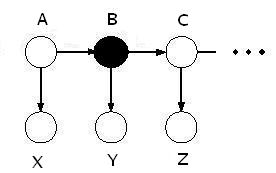
\includegraphics{./hmm/hmm-cond-ind.jpg}
  }
}
\end{figure}


\begin{proof}
\begin{eqnarray*}
p(a,b,c) &=& p(a)p(b|a)p(c|b)\\
p(c|a,b) &=& \frac{p(a,b,c)}{p(a,b)}\\
&=& \frac{p(a)p(b|a)p(c|b)}{p(a,b)}\\
&=& \frac{p(a)p(b|a)p(c|b)}{p(b|a)p(a)}\\
p(c|a,b) &=& p(c|b)
\end{eqnarray*}
\end{proof}

Also prove $X$ is independent of $Z$ given $B$.

\begin{figure}[!hbp]
\center{
  \scalebox{0.80}{
  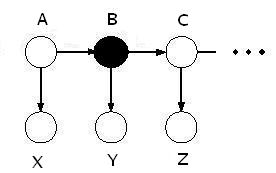
\includegraphics{./hmm/hmm-cond-ind.jpg}
  }
}
\end{figure}

\begin{proof}
\begin{eqnarray*}
p(a,b,c,x,y,z) &=& p(a)p(b|a)p(c|b)p(x|a)p(y|b)p(z|c)\\
p(a,c,y,z|b,x) &=& \frac{p(a,b,c,x,y,z)}{p(b,x)}\\
&=& \frac{p(a,b,c,x,y,z)}{\sum_a p(b,x|a)p(a)}\\
&=& \frac{p(a,b,c,x,y,z)}{ p(b,x|a)\sum_a p(a)}\\
&=& \frac{p(a,b,c,x,y,z)}{p(b|a)p(x|a)}\\
&=& \frac{p(a)p(b|a)p(c|b)p(x|a)p(y|b)p(z|c)}{p(b|a)p(x|a)}\\
&=& p(a)p(c|b)p(y|b)p(z|c)
\end{eqnarray*}

Hence, the fact that $x$ is given makes no difference in the joint distribution.

\end{proof}

We can use this to break up $p(y|q_t)$
